\documentclass[11pt]{article}
\usepackage{amssymb,graphicx,amsmath,mathtools,float}
\usepackage{lscape}
\usepackage[utf8]{inputenc}
\usepackage[spanish, es-tabla]{babel}

\usepackage{indentfirst}	% Tabular tras un section
\usepackage{hyperref}
\hypersetup{
	colorlinks,
	citecolor=black,
	filecolor=black,
	linkcolor=red,
	urlcolor=black
}

\usepackage[svgnames]{xcolor}
\definecolor{griscaption}{RGB}{100,100,100}
\usepackage{caption}
\usepackage[font={color=griscaption},figurename=Fig.,labelfont={bf}]{caption}


\newtheorem{theorem}{Theorem}
\newtheorem{corollary}[theorem]{Corollary}
\newtheorem{lemma}[theorem]{Lemma}
\newtheorem{proposition}[theorem]{Proposition}
\newtheorem{definition}[theorem]{Definición}


\title{Determinación de Órbitas Elípticas}
\author{Simón López
\\
{\small Matemáticas e Ingeniería Informática}
\\
{\small Universidad de Granada, 18071 Granada, Spain}
\\
{\small simondelosbros@correo.ugr.es}}
\date{\today}
\setlength{\unitlength}{1cm}
\setlength{\unitlength}{1cm}


\begin{document}


\section{Método Laplaciano de Determinación}

\subsection{\normalfont{\textit{Determinar el valor de la primera y segunda derivada de $\lambda$, $\mu$, $\nu$, $X$, $Y$, $Z$ en algún momento $t$.}}}
\label{primera_segunda_derivada}

Tomemos, por ejemplo, $t=t_2$, que por el momento nos bastará para demostrar que se puede realizar una buena aproximación. Supongamos que el valor de $\lambda'$ no cambia muy rápido; entonces, el valor de ésta en medio del intervalo $[t_1,t_2]$ será muy cercano al valor de:
\[
\lambda_{12}'=\frac{\lambda_2-\lambda_1}{t_2-t_1}
\]

Análogamente podremos determinar el valor de $\lambda_{23}'$; cuanto más pequeño sea el intervalo donde realizamos las operaciones, mejor será la aproximación obtenida. Además, si la longitud del intervalo $[t_1,t_2]$ es igual a la longitud de $[t_2,t_3]$, tenemos que el valor de $\lambda'$ en $t_2$ será muy cercano a:
\[
\lambda'_2=\frac{\lambda_{12}'+\lambda_{23}'}{2}
\]

\noindent es decir, la media de los dos valores calculados anteriormente. Si los intervalos tienen una longitud diferente, podremos ajustar la disparidad entre ellos.\\

Análogamente, podremos definir la derivada segunda de $\lambda$ en $t_2$ de manera aproximada como:
\[
\lambda''_2=\frac{\lambda_{23}'-\lambda_{12}'}{\frac{1}{2}(t_3-t_1)}
\]

Utilizaremos el mismo método para calcular la primera y segunda derivada de $\mu$ y $\nu$. Las aproximaciones obtenidas de esta manera serán más cercanas cuanto menor sea la longitud de los intervalos entre las observaciones, y generalmente, en la práctica, los intervalos que utilizaremos serán cortos.\\

Finalmente, para calcular la primera y segunda derivada de $X, Y$ y $Z$ utilizaremos el \textit{American Ephemeris}, que nos dará el valor de estas variables para cualquier día del año.\\

\subsection{\normalfont{\textit{Imponer la condición de que $C$ gira en torno a $S$ de acuerdo a la ley de gravitación.}}}
Asumiendo que el cuerpo observado $C$ no está alterado por la interacción con otros cuerpos cercanos, podemos asegurar que cumplirá siguientes ecuaciones diferenciales:
\begin{align}
\left\{
\begin{array}{l}
	\frac{d^2x}{dt^2}=-\frac{k^2x}{r^3}\\
	\frac{d^2y}{dt^2}=-\frac{k^2y}{r^3}\\
	\frac{d^2z}{dt^2}=-\frac{k^2z}{r^3}
\end{array}
\right.
\label{eq:ley_gracitacion_C}
\end{align}

\noindent donde $k^2=GM$, $G=6.674\times10^{-11}\frac{\text{N}\cdot\text{m}^2}{\text{kg}^2}$ constante de gravitación y $M=1.989\times10^{30}\;\text{kg}$ masa del Sol. Tomamos solo la masa del Sol, $M$, ya que la masa de nuestro cuerpo es despreciable en comparación con ésta.\\

Además, utilizando las \hyperref[eq:terminologia]{relaciones entre $E$, $C$ y $S$}, así como los resultados vistos anteriormente, llegamos a:
\begin{align}
\left\{
\begin{array}{l}
	x=\rho\lambda-X\\
	y=\rho\mu-Y\\
	z=\rho\nu-Z
\end{array}
\right.
\label{eq:relacion_C_S_E}
\end{align}

\noindent y sustituyendo los valores obtenidos en las  \hyperref[eq:ley_gracitacion_C]{ecuaciones \ref{eq:ley_gracitacion_C}}, obtenemos lo siguiente:
\begin{align}
\left\{
\begin{array}{l}
	(\rho\lambda)'' - X'' = \frac{-k^2(\rho\lambda-X)}{r^3}\\
	(\rho\mu)'' - Y'' = \frac{-k^2(\rho\mu-Y)}{r^3}\\
	(\rho\nu)'' - Z'' = \frac{-k^2(\rho\nu-Z)}{r^3}
\end{array}
\right.
\label{eq:derivada_segunda}
\end{align}

Desarrollando la segunda derivada de $\rho\lambda$ conseguimos:
\[
(\rho\lambda)''=(\rho'\lambda+\rho\lambda')'=\rho''\lambda+2\rho'\lambda'+\rho\lambda'',
\]

\noindent valor que utilizaremos más adelante.\\

De la misma manera que hemos hecho con $C$, escribimos las ecuaciones de gravitación para $E$, que gira alrededor de $S$ en concordancia con la ley de gravitación universal.
\begin{align}
\left\{
\begin{array}{l}
	X'' = -\frac{k^2X}{R^3}\\
	Y'' = -\frac{k^2Y}{R^3}\\
	Z'' = -\frac{k^2Z}{R^3}
\end{array}
\right.
\label{eq:ley_gravitacion_E}
\end{align}\\

Utilizando este resultado, sustituyendo en la ecuación \ref{eq:derivada_segunda} y desarrollando llegamos a lo siguiente:
\begin{align}
\left\{
\begin{array}{l}
	\lambda\rho''+2\lambda'\rho'+[\lambda''+\frac{k^2\lambda}{r^3}]\rho=-k^2X[\frac{1}{R^3}-\frac{1}{r^3}]\\
	\mu\rho''+2\mu'\rho'+[\mu''+\frac{k^2\mu}{r^3}]\rho=-k^2Y[\frac{1}{R^3}-\frac{1}{r^3}]\\
	\nu\rho''+2\nu'\rho'+[\nu''+\frac{k^2\nu}{r^3}]\rho=-k^2Z[\frac{1}{R^3}-\frac{1}{r^3}]
\end{array}
\right.
\label{eq:fin_paso_1}
\end{align}

Así, las incógnitas de las ecuaciones pasan a ser $r, \; \rho, \; \rho'$ y $\rho''$.\\

\subsection{\normalfont{\textit{Determinar la Distancia de $C$ desde $E$ y $S$}}}
Para resolver este paso, utilizaremos las ecuaciones que hemos acabado obteniendo del paso anterior, \ref{eq:fin_paso_1}, y una condición geométrica que cumplirán los tres cuerpos. Para ello, tomaremos el sistema \ref{eq:fin_paso_1} como un sistema lineal en $\rho, \rho'$ y $\rho''$ y resolveremos utilizando la regla de Cramer. Comencemos definiendo el siguiente determinante:

\[
D =
\left|
\begin{array}{ccc}
	\lambda & 2\lambda' & \lambda''+\frac{k^2\lambda}{r^3}\\
	\mu & 2\mu' & \mu''+\frac{k^2\mu}{r^3}\\
	\nu & 2\nu' & \nu''+\frac{k^2\nu}{r^3}
\end{array}
\right|
=
2
\left|
\begin{array}{ccc}
	\lambda & \lambda' & \lambda''\\
	\mu & \mu' & \mu''\\
	\nu & \nu' & \nu''
\end{array}
\right|
\]

Esta segunda forma del determinante la obtenemos mediante la transformación $C_3-\frac{k^2\lambda}{r^3}C_1$ sobre la matriz, donde $C_i$ será la columna i-ésima. En este determinante conocemos todos las cantidades.\\

Por otra parte, definiremos el determinante $D_1$, que utilizaremos para calcular $\rho$ mediante la regla de Cramer, reemplazando la tercera columna por el miembro de la derecha de las \hyperref[eq:fin_paso_1]{ecuaciones anteriores} y omitiendo el factor $[\frac{1}{R^3}-\frac{1}{r^3}]$, conociendo de nuevo todas las cantidades utilizadas. Así, obtenemos el siguiente determinante:

\[
D_1 = -2k^2
\left|
\begin{array}{ccc}
\lambda & \lambda' & X\\
\mu & \mu' & Y\\
\nu & \nu' & Z
\end{array}
\right|
\]\\

Con todo esto, la distancia $\rho$ se determina por

\[
\rho = \frac{D_1}{D}[\frac{1}{R^3}-\frac{1}{r^3}],
\]

El valor de $r$ es desconocido, por lo que añadiremos la siguiente ecuación formando con las dos un sistema de ecuaciones en $r$ y $\rho$

\[
r^2=\rho^2+R^2-2\rho R\cos(\psi),
\]

\noindent donde $\psi$ es el ángulo en $E$ entre $r$ y $\rho$; esta ecuación expresa el hecho de que $S$, $E$ y $C$ forman un triángulo como vimos en la \hyperref[figure:1]{figura 1}. Resolviendo el sistema de ecuaciones al que hemos llegado obtendremos los valores de $\rho$ y $r$, habiendo terminado este paso. Al solucionar este problema, podremos calcular las coordenadas de $C$ mediante las ecuaciones de \hyperref[eq:relacion_C_S_E]{las relaciones} entre $S$, $E$ y $C$.\\

\subsection{\normalfont{\textit{Determinación de las Componentes de Velocidad de $C$}}}
Se sigue de las ecuaciones \ref{eq:relacion_C_S_E} que:
\[
\left\{
\begin{array}{l}
	x'=\rho'\lambda+\rho\lambda'-X'\\
	y'=\rho'\mu+\rho\mu'-Y'\\
	z'=\rho'\nu+\rho\nu'-Z'
\end{array}
\right.	
\]

En estas ecuaciones solo tenemos una incógnita, $\rho'$, que podremos determinar resolviendo por Cramer, al igual que en el anterior paso, a partir de:

\[
\rho'=+\frac{D_2}{D}[\frac{1}{R^3}-\frac{1}{r^3}],
\; \; \; \; \; \; \; \; \; \text{ con } \;
D_2 = -k^2
\left|
\begin{array}{ccc}
\lambda & X & \lambda''\\
\mu & Y & \mu''\\
\nu & Z & \nu''
\end{array}
\right|
\]


Así, $x'$, $y'$ y $z'$ se vuelven conocidas.\\

\subsection{\normalfont{\textit{Determinar los elementos de la órbita a partir de la posición y los componentes de velocidad del cuerpo observado}}}
Una vez conocida tanto la posición como la velocidad del cuerpo en un instante determinado, nos dispondremos a calcular los elementos orbitales mediante las distintas fórmulas estudiadas en el manual de Mecánica Celeste\cite{ortega}. Denotemos por $x(t)=(x,y,z)(t)$ la posición del objeto y $x'(t)$ su derivada, la velocidad.

Comencemos determinando la energía que tiene nuestro cuerpo en un instante $t$. Para ello utilizaremos:

\[
h=\frac{|x'(t)|^2}{2}-\frac{\mu}{|x(t)|}
\]

\noindent donde $\mu=GM$ una constante positiva. Con el valor de la energía podemos pasar a calcular la primera de nuestros elementos astronómicos, la longitud del semieje mayor, $a$, utilizando la siguiente ecuación:

\[
a=-\frac{\mu}{2h}
\]

Pasemos ahora a calcular el momento angular de nuestro objeto. Dado que la masa del objeto observado es despreciable frente a la masa del Sol, podremos obviar su valor, obteniendo así el vector del momento angular mediante:
\[
c=x(t)\wedge x'(t)
\]

Calculado el momento angular, podremos obtener el vector de excentricidad para la órbita del cuerpo observado:
\[
\vec{e}=-\frac{x(t)}{|x(t)}-\frac{1}{\mu}(c\wedge x'(t))
\]

\noindent y la excentricidad de la órbita será $e=|\vec{e}|$.\\

Una vez obtenidos estos valores, podemos utilizar la tercera ley de Kepler para obtener el período mínimo (suponiendo que nuestra órbita se corresponda con la de una elipse). Si el momento angular del objeto observado $c\neq0$ y su energía $h<0$, entonces la órbita es periódica y su período mínimo valdrá:
\[
p=\frac{2\pi}{\sqrt{\mu}}a^{3/2}
\]

Sabemos que el vector del momento angular, del que disponemos, es el vector normal al plano orientado de la órbita, pudiendo calcular así la inclinación del plano de movimiento. Además, calculando la intersección de éste con el plano de la eclíptica obtenemos la línea de nodos $\mathcal{N}_+$, con la que podremos determinar $\Omega$.
\[
\left\{
\begin{array}{l}
	i=\measuredangle(\vec{e}_3,\vec{n}), \; \; \; \; \; \; \; \; \; \; i\in]0,\pi[\\
	\Omega=\measuredangle(\vec{e}_1, \mathcal{N}_+), \; \; \; \; \; \Omega\in\mathbb{R}/2\pi\mathbb{Z}
\end{array}
\right.
\]

Finalmente usaremos el vector de excentricidad $\vec{e}$ para calcular $\omega$, usando la línea de nodos como eje de rotación.\\

\subsection{\normalfont{\textit{Determinación de $\lambda$, $\mu$ y $\nu$ y sus derivadas mediante series de potencias}}}

Tal y como hemos visto en la sección \ref{primera_segunda_derivada}, hemos de calcular la primera y segunda derivada de las coordenadas angulares o de $\lambda$, $\mu$ y $\nu$. Veamos un método de cálculo diferente. Para ello, comencemos definiendo el valor $\tau=k(t-t_0)$, pudiendo reescribir las ecuaciones \ref{eq:ley_gracitacion_C} como vemos a continuación:
\begin{align}
\left\{
\begin{array}{l}
	\frac{d^2x}{d\tau^2}=-\frac{x}{r^3}\\
	\frac{d^2y}{d\tau^2}=-\frac{y}{r^3}\\
	\frac{d^2z}{d\tau^2}=-\frac{z}{r^3}
\end{array}
\right.
\label{eq:ley_gracitacion_C_2}
\end{align}

La solución para estas ecuaciones diferenciales de segundo orden puede ser expandida como serie de Taylor en $\tau$, y esta convergerá si el valor de $\tau$ no es especialmente grande.
\begin{align}
\left\{
\begin{array}{l}
	x=x_0+x_0'\tau+\frac{1}{2}(\frac{d^2x}{d\tau^2})_0\tau^2+...+\frac{1}{n!}(\frac{d^nx}{d\tau^n})_0\tau^n+...\\
	y=y_0+y_0'\tau+\frac{1}{2}(\frac{d^2y}{d\tau^2})_0\tau^2+...+\frac{1}{n!}(\frac{d^ny}{d\tau^n})_0\tau^n+...\\
	z=z_0+x_0'\tau+\frac{1}{2}(\frac{d^2z}{d\tau^2})_0\tau^2+...+\frac{1}{n!}(\frac{d^nz}{d\tau^n})_0\tau^n+...\\	
\end{array}
\right.
\label{eq:series_taylor}
\end{align}

\noindent donde con el subíndice 0 estaremos indicando que los valores se toman en $\tau=0$. Podemos sustituir la segunda derivada que aparece en estas series por su valor en \ref{eq:ley_gracitacion_C_2}, la tercera derivada por la derivada de ésta y a partir de la cuarta derivada repetimos este proceso, teniendo así que las series estarán solo en función de la $x$, $y$, $z$ y la primera derivada de cada una de estas, todos ellas tomadas en $\tau=0$.\\

Hemos de tener en cuenta que el valor de estas series no siempre tiene valor práctico, pues el intervalo de tiempo para la convergencia puede ser demasiado grande; notar que los límites serán más pequeños cuanto más pequeña sea la distancia del perihelio y más grande la excentricidad de nuestra órbita, y dependerán de la posición del cuerpo en $\tau=0$.\\

En el caso de la Tierra, expandiendo sus coordenadas en series de potencias, obtendremos una convergencia durante largos intervalos de tiempo debido a la pequeña excentricidad de la órbita terrestre ($e\approx0.0167$). Así, se sigue de la ecuación \ref{eq:relacion_C_S_E}, que relaciona las coordenadas de la Tierra, el Sol y el cuerpo observado que las ecuaciones de $\rho$, $\lambda$, $\mu$ y $\nu$ también podrán ser expandidas como series de Taylor, con el mismo rango de utilidad que el de las series para $x$, $y$ y $z$.\\

Veamos las series para $\lambda$, pues las de $\mu$ y $\nu$ serán simétricamente similares. Definimos $\tau_1$, $\tau_2$ y $\tau_3$ como los valores de $\tau$ tomando $t_1$, $t_2$ y $t_3$ respectivamente. Así, las series para $\lambda$ son:
\begin{align}
\left\{
\begin{array}{l}
\lambda=c_0+c_1\tau+c_2\tau^2+...\\
\lambda_1=c_0+c_1\tau_1+c_2\tau_1^2+...\\
\lambda_2=c_0+c_1\tau_2+c_2\tau_2^2+...\\
\lambda_3=c_0+c_1\tau_3+c_2\tau_3^2+...
\end{array}
\right.
\label{eq:series_lambda}
\end{align}

\noindent donde los valores $c_0, c_1, c_2, ...$ son constantes. Si estas series terminan tras los términos elevados al cuadrado, podremos determinar $c_0$, $c_1$ y $c_2$ resolviendo un sistema de ecuaciones, ya que conocemos las cantidades observadas $\lambda_1$, $\lambda_2$, $\lambda_3$. Así, tenemos que cuantas más observaciones tengamos disponibles, más coeficientes podrán ser determinados.\\

Para expresar $\lambda$ en términos de $\tau$ tomando solo coeficientes conocidos, igualaremos a 0 la resultante de $1$, $c_0$, $c_1$ y $c_2$, y obtendremos lo siguiente:
\begin{align}
\left|
\begin{array}{cccc}
\lambda & 1 & \tau & \tau^2\\
\lambda_1 & 1 & \tau_1 & \tau^2_1\\
\lambda_2 & 1 & \tau_2 & \tau^2_2\\
\lambda_3 & 1 & \tau_3 & \tau^2_3\\
\end{array}
\right|
=0
\label{eq:resultante}
\end{align}

Resolvemos este determinante desarrollando por la primera columna y despejando $\lambda$ obtenemos:
\begin{align}
\lambda=
\frac{(\tau-\tau_2)(\tau-\tau_3)}{(\tau_1-\tau_2)(\tau_1-\tau_3)}\lambda_1
+\frac{(\tau-\tau_3)(\tau-\tau_1)}{(\tau_2-\tau_3)(\tau_2-\tau_1)}\lambda_2
+\frac{(\tau-\tau_1)(\tau-\tau_2)}{(\tau_3-\tau_1)(\tau_3-\tau_2)}\lambda_3
\label{eq:lambda_value}
\end{align}

\noindent donde hemos de tener en cuenta que los valores de $\tau_1$, $\tau_2$ y $\tau_3$ han de ser diferentes entre sí para que no se anulen los denominadores.\\

Con esto, somos capaces de obtener $\lambda$ de manera exacta en $\tau_1$, $\tau_2$ y $\tau_3$; para otros valores más pequeños de $\tau$ obtendremos $\lambda$ de forma aproximada. Para obtener un valor exacto de $\lambda$ habremos de tomar la primera ecuación de \ref{eq:series_lambda}, una serie infinita, dentro de su rango de convergencia. Considerando esta serie geométricamente podemos definir una curva que llamaremos $C$; por otra parte definiremos la curva $C_2$ como la que produce el polinomio \ref{eq:lambda_value}. Representando las dos en una misma gráfica podemos visualizar lo siguiente:
\begin{figure}[H]
\centering
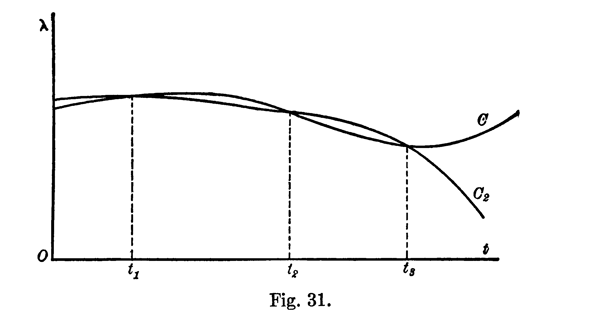
\includegraphics[scale=0.5]{images/fig_31.png}
\end{figure}

Dichas curvas se intersecan en $\tau_1$, $\tau_2$ y $\tau_3$, y en general en ningún otro punto; tomando valores pequeños de $\tau$ las dos curvas casi coincidirán.\\

Por último, ya que necesitamos la primera y segunda derivada de $\lambda$, nos bastará con derivar de la ecuación \ref{eq:lambda_value}.
\begin{align*}
\lambda' = \frac{2\tau-(\tau_2+\tau_3)}{(\tau_1-\tau_2)(\tau_1-\tau_3)}\lambda_1
+\frac{2\tau-(\tau_3+\tau_1)}{(\tau_2-\tau_3)(\tau_2-\tau_1)}\lambda_2
+\frac{2\tau-(\tau_1+\tau_2)}{(\tau_3-\tau_1)(\tau_3-\tau_2)}\lambda_3\\
\lambda'' = \frac{2}{(\tau_1-\tau_2)(\tau_1-\tau_3)}\lambda_1
+\frac{2}{(\tau_2-\tau_3)(\tau_2-\tau_1)}\lambda_2
+\frac{2}{(\tau_3-\tau_1)(\tau_3-\tau_2)}\lambda_3
\end{align*}

Tal y como comentamos anteriormente, se procederá al cálculo de $\mu$ y $\nu$ de manera similar a la desarrollada anteriormente.



\newpage

\begin{thebibliography}{99}
\bibitem{moulton} \textsc{Forest Ray Moulton}, \textsc{An Introduction to Celestial Mechanics}, \textit{second edition}.

\bibitem{ortega} \textsc{R. Ortega, A.J. Ureña}, \textsc{Introducción a la Mecánica Celeste}.

\bibitem{right_ascension_declination} \textsc{Sky \& Telescope}, \textsc{Right Ascension and Declination: Celestial Coordinates For Beginners}, \url{https://skyandtelescope.org/astronomy-resources/right-ascension-declination-celestial-coordinates/}

\end{thebibliography}

\end{document}
